
\section{Experiments}
%------------------------------------------------

% \begin{frame}{Single images}
%    \begin{figure}[h]
%        \centering
%        
\includegraphics[width=0.7\textwidth]{img/logo_v2.png}
%        \caption{Slide with single images}
%        \label{fig:sing_image}
%    \end{figure}
% \end{frame}

% %------------------------------------------------

% \begin{frame}{Single image with itemize}
%      Lorem ipsum dolor sit amet, consectetur adipiscing elit:
%     \begin{enumerate}
%         \item Lorem ipsum dolor sit amet.
%         \item Lorem ipsum dolor sit amet.
%     \end{enumerate}
    
%    \begin{figure}[h]
%        \centering
%        
\includegraphics[width=0.7\textwidth]{img/logo_v2.png}
%        \caption{Slide with single images}
%        \label{fig:sing_image}
%    \end{figure}
% \end{frame}

%------------------------------------------------
\begin{frame}{Methodology}

\begin{columns}

\column{0.3\textwidth}
 \footnotesize
    \begin{thebibliography}{99}
        \bibitem{autorlivro} Zhang, Yinghua, et al. "Two sides of the same coin: White-box and black-box attacks for transfer learning." Proceedings of the 26th ACM SIGKDD international conference on knowledge discovery \& data mining. 2020.

    \end{thebibliography}

\column{0.7\textwidth}
    \begin{figure}
        \begin{subfigure}{0.9\textwidth}
            \centering
            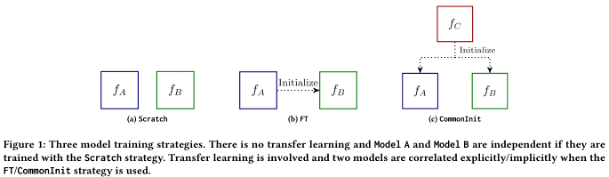
\includegraphics[scale=0.55]{img/exper-1.png}
     
            \label{fig:sub-figure-url-1}
        \end{subfigure} \\
        \begin{subfigure}{0.9\textwidth}
            \centering
            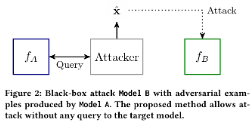
\includegraphics[scale=0.55]{img/exper-2.png}
    
            \label{fig:sub-figure-url-2}
        \end{subfigure}
        \label{fig:example-subfigure}
    \end{figure}
    \begin{itemize}
        \item Datasets: MNIST (M), USPS (U), SVHN (S), SynDigits (Syn), CIFAR10, STL10, ImageNet32
    \end{itemize}
\end{columns}

\end{frame}

%------------------------------------------------
\begin{frame}{White-box Attack Experiment}
\begin{columns}[T]
    \column{0.4\textwidth}
        \begin{itemize}
            \item \textbf{Goal}: Assess robustness to FGSM attacks.
            \item \textbf{Method}: Compare Scratch vs. Fine-tuning models under various noise levels.
            \item \textbf{Result}:
            \begin{itemize}
                \item Fine-tuning significantly improves accuracy and robustness.
                \item Example: Accuracy increases from 50.86\% -> 84.96\% at $\epsilon = 0.125$.
            \end{itemize}
            % \item \textbf{Conclusion}: Fine-tuning enhances both performance and security.
        \end{itemize}

    \column{0.6\textwidth}
       \begin{figure}[h]
           \centering
           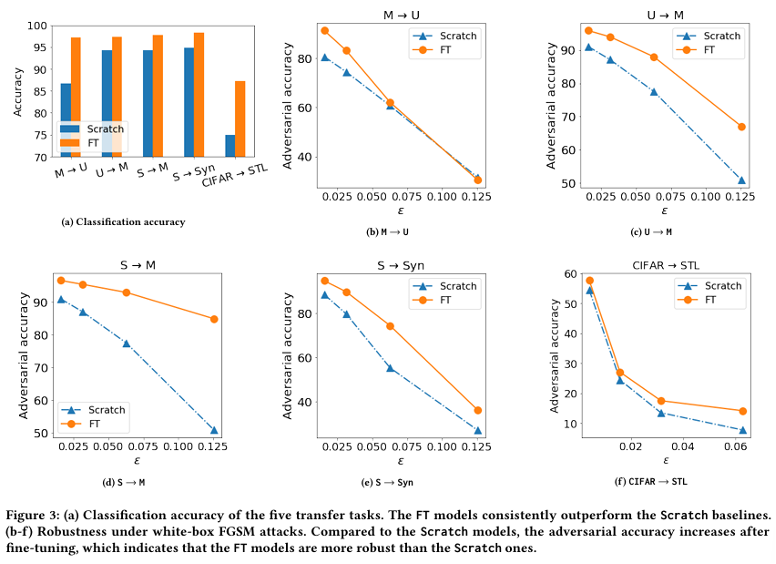
\includegraphics[scale=0.7]{img/white-box.png}
           \label{fig:what-is}
       \end{figure}
    \end{columns}
\end{frame}
%------------------------------------------------
\begin{frame}{Black-box Attack Experiment}
\begin{columns}[T]
    \column{0.6\textwidth}
       \begin{figure}[h]
           \centering
           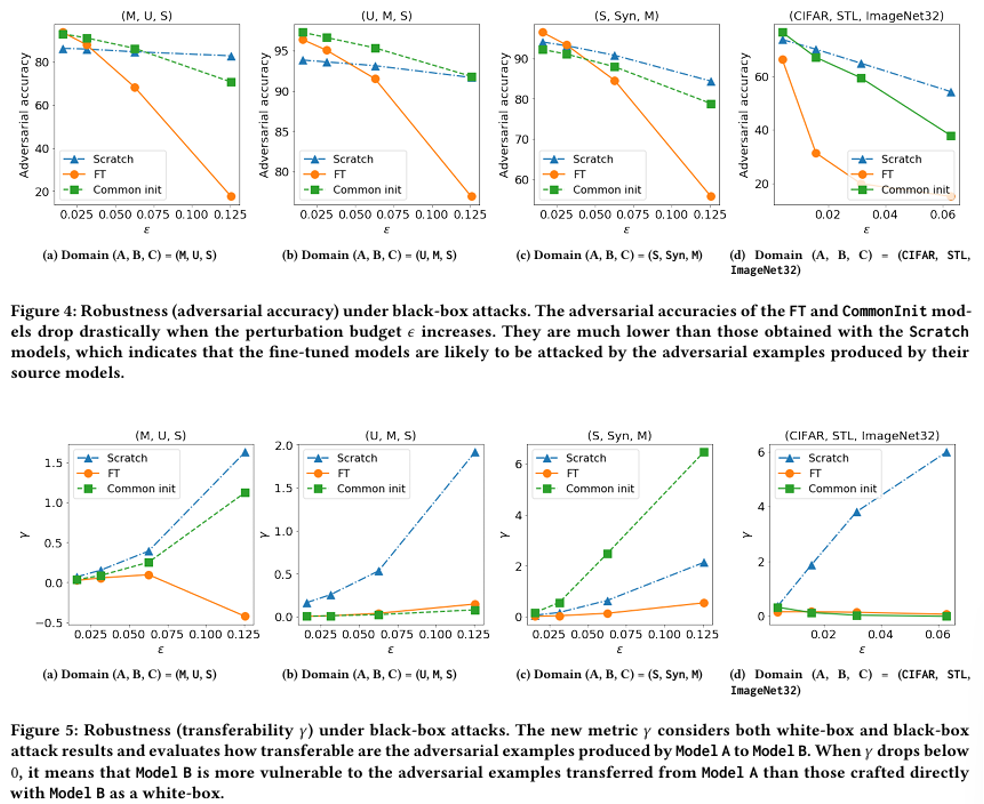
\includegraphics[scale=0.5]{img/black-box.png}
           \label{fig:black-box}
       \end{figure}
    \column{0.4\textwidth}
        \begin{itemize}
            \item \textbf{Goal}: Evaluate transferability of adversarial examples.
            \item \textbf{Method}: Attack model B using adversarial examples from model A.
            \item \textbf{Result}:
            \begin{itemize}
                \item Fine-tuned models are more vulnerable to transferred attacks.
                \item Example: Accuracy drops from 87.43\% -> 65.32\% (FGSM).
            \end{itemize}
            % \item \textbf{Conclusion}: Fine-tuning improves performance but increases attack susceptibility.
        \end{itemize}
\end{columns}
\end{frame}

%------------------------------------------------